\newpage
\section{Решения уравнений Максвелла}
    В этой главе рассматриваются следующие уравнения:
    \begin{gather*}
        \rot\vec{H} = \frac{1}{c}\pard{\vec{E}}{t} + \frac{4\pi}{c}\vec{j}, \: \Div\vec{H} = 0,\\
        \rot\vec{E} = -\frac{1}{c}\pard{\vec{H}}{t}, \:\: \Div\vec{E} = 4\pi\rho,\\
        \vec{E} = -\frac 1c \pard{\vec{A}}{t} - \nabla\phee, \:\: \vec{H} = \rot\vec{A}.
    \end{gather*}
\subsection{Статические и квазистационарные поля}
    Рассмотрим относительно простой случай, при котором поля не меняются в зависимости от времени.
        \begin{numcases}{}
            \vec{E} = -\nabla\phee \label{elstat1} \\
            \Div\vec{E} = 4\pi\rho \label{elstat2} \\
            \rot\vec{E} = 0 \label{elstat3}
        \end{numcases}
        \begin{numcases}{}
            \vec{H} = \rot\vec{A} \label{magstat1}\\
            \Div\vec{H} = 0 \label{magstat2}\\
            \rot\vec{H} = \frac{4\pi}{c}\vec{j} \label{magstat3}
        \end{numcases}

    Уравнения распались на электрическую и магнитную части. Отметим, что из уравнения (\ref{elstat1}) автоматически следует
    уравнение (\ref{elstat3}). Подставим (\ref{elstat1}) в (\ref{elstat2}), чтобы получить
    \[\boxed{
        \Delta\phee = -4\pi\rho}
    \]
    что есть уже знакомое нам уравнение Пуассона. Аналогично и с уравнениями на магнитное поле: равенство (\ref{magstat2}) получается
    как следствие из (\ref{magstat1}). Подстановкой (\ref{magstat1}) в (\ref{magstat3}) мы получим
    \[
        \rot\rot\vec{A} = \grad\Div\vec{A} - \Delta\vec{A} = \frac{4\pi}{c}\vec{j}.
    \]
    Налагая на векторный потенциал калибровочное условие $\Div\vec{A} = 0$, получаем уравнение Пуассона для векторного потенциала:
    \begin{equation}\boxed{
        \Delta\vec{A} = -\frac{4\pi}{c}\vec{j}} \label{mag_Poisson}
    \end{equation}
    Найдём решения уравнения Пуассона для точечной частицы. Поместим частицу в начало координат, в этом случае $\rho(\vec{r}) = e\delta(\vec{r})$.
    Уравнение Пуассона запишется так:
    \[
        \Delta\phee = -4\pi e\delta(\vec{r})
    \]
    Правая часть представляет собой сферически симметричную функцию, поэтому и потенциал мы будем искать сферически симметричный.
    Проинтегрируем левую часть по сферическому объёму $\vol$ и воспользуемся теоремой Гаусса-Остроградского:
    \begin{gather*}
        \int_{\vol}\Delta\phee d\vol = \int_{\vol}\Div\grad\phee d\vol = 
        \oint_{S}\grad\phee d\vec{f} = \frac{d\phee}{dr}\cdot 4\pi r^2.
    \end{gather*}
    В силу сферической симметрии на сфере радиуса $r$ потенциал $\phee$ и $\grad\phee$ постоянны. Интеграл правой части
    \[
        \int_{\vol} 4\pi e\delta(\vec{r})d\vol = 4\pi e.
    \]
    Получаем соотношение
    \[
        \frac{d\phee}{dr} = -\frac{e}{r^2},
    \]
    из которого следует известное выражение для кулоновского потенциала:
    \[
        \boxed{\phee(r) = \frac{e}{r} + const}
    \]
    \begin{note}
        Мы получили важное математическое соотношение:
        \begin{equation}
            \Delta\brackets{\frac 1r} = -4\pi \delta(\vec{r}) \label{ImportantEquation}
        \end{equation}
        Формальное дифференцирование в этом случае дало бы неверный результат $\Delta\brackets{\frac 1r} \equiv 0$
    \end{note}
    
    Для заряда в произвольной точке пространства $r_a$ верно: $\rho(\vec{r}) = e\delta\brackets{\vec{r} - \vec{r}_a}$, а потенциал заряда равен
    \[
        \phee(\vec{r}) = \frac{r}{\abs{\vec{r} - \vec{r}_a}}.
    \]
    в силу принципа суперпозиции для нескольких зарядов имеем
    \begin{equation}
        \phee(\vec{r}) = \sum_{a=1}^N \frac{e_a}{\abs{\vec{r} - \vec{r}_a}}. \label{potent_sum}
    \end{equation}
    Решение (\ref{potent_sum}) можно распространить на случай непрерывного распределения заряда в пространстве:
    \[
        \phee(\vec{r}) = \sum_a \int \frac{e_a\delta(\vec{r'} - \vec{r}_a)d \vol '}{\abs{\vec{r} - \vec{r'}}} = \int \frac{\sum_a e_a\delta(\vec{r'} - \vec{r}_a)d \vol '}{\abs{\vec{r} - \vec{r'}}} =
        \int \frac{\rho(\vec{r'})}{\abs{\vec{r} - \vec{r'}}} d\vol'
    \]
    Здесь $d\vol' = d^3(\vec{r'})$, интегрирование ведётся по всему исследуемому пространству.

    Ограничимся рассмотрением только тех задач, где плотность заряда $\rho(\vec{r'})$ уже задана. Даже в этом случае нахождение общего решения затруднительно.

\subsection{Электростатическое поле на больших расстояниях от системы}
    \begin{figure}[h]
        \centering{
            \begin{tikzpicture}
    \draw [->] (0, 0) -- (6, 0) node [anchor = north] {$Z$};
    \draw [->] (0, 0) -- (0, 4) node [anchor = west] {$X$};
    \draw [->] (0, 0) -- (-1.5, -1.5) node [anchor = north west] {$Y$};
    \draw [thick, blue] (0, 0) circle(0.85cm);
    \filldraw [black] (5.5, 3) circle (1.5pt);
    \filldraw [black] (0.5, -0.5) circle (1.5pt);
    \draw [->] (0,0) -- (0.5, -0.5) node [above] {$\vec{r}'$};
    \filldraw [black] (5.5, 3) circle (1.5pt);
    \draw [->] (0,0) -- (5.5, 3) node [above, midway] {$\vec{r}$};
    \draw [->] (0.5, -0.5) -- (5.5, 3) node [below, midway] {$\vec{r} - \vec{r}'$};
    \filldraw [black] (0.1, 0.4) circle (0.8pt);
    \filldraw [black] (-0.1, -0.4) circle (0.8pt);
    \filldraw [black] (-0.4, -0.2) circle (0.8pt);
    \filldraw [black] (0.1, -0.4) circle (0.8pt);
    \draw [->] (-1.2, 1.2) -- (-0.6, 0.6) node [above, midway] {$l$};
    \draw [->] (1.2, -1.2) -- (0.6, -0.6);
\end{tikzpicture}
        }
    \end{figure}

    Поместим рассматриваемую систему в начало координкт, как на рисунке. Пусть все растояния до зарядов системы $\vec{r'}$ не превосходят некоторой величины $l$ ---
    характерного размера системы. Выберем точку наблюдения $\vec{r}$ так, что $\abs{\vec{r}} \gg l$, тогда $\abs{\vec{r'}} \sim l \ll \abs{\vec{r}}$. Задача состоит в
    нахождении потенциала
    \begin{equation}
        \phee{\vec{r}} = \int \frac{\rho(\vec{r'} d\vol')}{\abs{\vec{r} - \vec{r'}}}. \label{potent_int}
    \end{equation}
    Рассмотрим знаменатель выражения под интегралом:
    \begin{gather}
        \frac{1}{\abs{\vec{r} - \vec{r'}}} = \frac{1}{\sqrt{r^2 - 2\dotp{r}{r'} + (r')^2}} = \frac{1}{r} \brackets{1 - 2\frac{\dotp{r}{r'}}{r^2} + \brackets{\frac{r'}{r}}^2} \notag \\
        \approx \frac{1}{r}\brackets{1 + \frac{\dotp{r}{r'}}{r^2} - \frac{(r')^2}{2r^2} + \frac{3}{2} \frac{\dotp{r}{r'}^2}{r^4}} = 
        \frac{1}{r} + \frac{\dotp{r}{r'}}{r^3} + \frac{x_{\alpha} x_{\beta} \brackets{3x_{\alpha}'x_{\beta}' - (r')^2 \delta_{\alpha\beta}}}{2r^5} \label{multipole_series}
    \end{gather}
    Поясним, откуда получилось последнее выражение:
    \begin{gather*}
        x_{\alpha}x_{\alpha}' = \dotp{r}{r'} = x_{\beta}x_{\beta}' \: \Rightarrow \: x_{\alpha}x_{\beta} \cdot 3x_{\alpha}'x_{\beta}' = 3\dotp{r}{r'};\\
        x_{\alpha} x_{\beta}\delta_{\alpha\beta} = x_{\alpha}x_{\alpha} = (\vec{r})^2.
    \end{gather*}
    Подставим выражение (\ref{multipole_series}) в (\ref{potent_int}):
    \begin{gather*}
        \phee(\vec{r}) = \frac 1r \int \rho(\vec{r'}) d\vol' + \frac{\vec{r'}}{r^3}\int \vec{r'}\rho(\vec{r'}) d\vol' + \frac{x_{\alpha}x_{\beta}}{2r^5}\int\rho(\vec{r'})
        \brackets{3x_{\alpha}'x_{\beta}' - \delta_{\alpha\beta}(\vec{r'})^2}d\vol'.
    \end{gather*}
    Учитывая $\int \rho(\vec{r'}) d\vol' = e = \sum_a e_a$ и $\int \rho(\vec{r'}) \vec{r'} d\vol' = \sum_a e_a\vec{r}_a = \vec{d}$, получаем
    \begin{equation}
        \phee(\vec{r}) \frac er + \frac{\dotp{d}{r}}{r^3} + \frac{x_{\alpha}x_{\beta} D_{\alpha\beta}}{r^5}. \label{quad_potent}
    \end{equation}
    Тензор $D_{\alpha\beta}$ в случае непрерывного и дискретного распределения равен, соответственно,
    \begin{gather*}
        D_{\alpha\beta} = \int\rho(\vec{r'})\brackets{3x_{\alpha}'x_{\beta}' - \delta_{\alpha\beta}(r')^2}d^3\vec{r'};\\
        D_{\alpha\beta} = \sum_a e_a \brackets{3{x_{\alpha}^{(a)}}' {x_{\beta}^{(a)}}' - \delta_{\alpha\beta}(r')^2}.
    \end{gather*}
    Выражение (\ref{quad_potent}) представляет собой \textit{мультипольное разложение} по малому параметру $l$, которое в нашем случае состоит из дипольного и квадрупольного членов.
    Выражение для дипольного электрического поля уже было нами получено:
    \begin{gather*}
        \vec{E}_{\vec{d}} = -\nabla\phee = -\nabla\frac{\dotp{d}{r}}{r^3} = -\frac{\nabla\dotp{d}{r}}{r^3} - \dotp{d}{r}\nabla\frac{1}{r^3} = \\
        = -\frac{\vec{d}}{r^3} + \frac{3\dotp{d}{r}\vec{r}}{r^5} = \Biggm| \vec{n} = \frac{\vec{r}}{\abs{\vec{r}}} \Biggm| = \frac{3\dotp{d}{n} - \vec{d}}{r^3}.
    \end{gather*}

    Тензор $D_{\alpha\beta}$ называется \textit{тензором квадрупольного момента}. Его свойства:
    \begin{itemize}
        \item Симметричность: $D_{\alpha\beta} = D_{\beta\alpha}$;
        \item Нулевой след: 
            \[
                \trace D_{\alpha\beta} = D_{\alpha\alpha} = 3x_{\alpha}'x_{\alpha}' - \delta_{\alpha\alpha}(\vec{r'})^2 = 3(r')^2 - 3(r')^2 = 0.
            \]
    \end{itemize}
    В силу вышеуказанных свойств этот тензор имеет всего 5 независимых компонент. Также $D_{\alpha\beta}$ можно привести к диагональному виду:
    \[
        D_{\alpha\beta} = \begin{bmatrix}
            D_{xx} & 0 & 0 \\
            0 & D_{yy} & 0 \\
            0 & 0 & D_{zz}
        \end{bmatrix}
    \]
    В этом виде тензор имеет всего две независимые компоненты.

        \parbox[h]{3cm}{
            \begin{tikzpicture}
    \draw (0,0) ellipse (1.2 and 2);
    \draw (0,0) ellipse (1.2 and 0.6);
    \draw [->] (0,0) -- (0, 2.6) node [anchor = west] {$Z$};
    \draw [->] (0,0) -- (2, 2.4) node [anchor = south west] {$\vec{r}$};
    \coordinate (g1) at (0,1);
    \coordinate (g2) at (1, 1,2);
    \coordinate (q) at (0,0);
    \pic [draw] {angle = g2--q--g1};
    \node [] at (0.2, 0.7) {$\theta$};
\end{tikzpicture}
        }
        \hfill
        \parbox[h]{12cm}{
            Если система имеет аксиальную симметрию, например, относительно оси $z$ (см. рисунок), то
            \[
                D_{xx} = D_{yy} = -\frac 12 D_{zz}.
            \]
        }
    
    В этом случае величина $D_{zz} \equiv D$ называется \textit{квадрупольным моментом} системы. Квадрупольный потенциал симметричной системы равен
    \begin{gather*}
        \phee_D = \frac{n_{\alpha}n_{\beta}D_{\alpha\beta}}{2r^3} = \frac{-\frac D2 \brackets{n_x^2 + n_y^2} + Dn_z^2}{2r^3} =
        \frac{D\brackets{\cos^2\theta - \frac{\sin^2\theta}{2}}}{2r^3} = \frac{D\brackets{3\cos^2\theta - 1}}{4r^3}.
    \end{gather*}
    Здесь $\theta$ --- угол между вектором $\vec{r}$ и осью $z$ в вертикальной плоскости.
    \begin{note}
        \[
            \phee_D(\vec{r}) = \frac{D}{2r^3}P_2(\cos\theta),
        \]
        где $\displaystyle P_2(x) = \frac{3x^2 - 1}2$ --- полином Лежандра второго порядка.
    \end{note}

\subsection{Энергия системы зарядов}
    По существу, это энергия создаваемого электромагнитного поля с плотностью $w = \frac{E^2}{8\pi}$. Полная потенциальная энергия равна
    \[
        U = \iiint \frac{E^2}{8\pi}d\vol = -\frac{1}{8\pi} \iiint \dotp{E}{\nabla}\phee d\vol.
    \]
    Используем соотношение $\Div\brackets{\vec{E}\phee} = \phee\Div\vec{E} + \vec{E}\nabla\phee$:
    \[
        U = -\frac{1}{8\pi}\int\Div\brackets{\vec{E}\phee} d\vol + \frac{1}{8\pi}\int\phee\Div\vec{E}d\vol.
    \]
    Если система зарядов ограничена в пространстве, то по теореме Гаусса-Остроградского получаем
    \[
        \int \Div\brackets{\vec{E}\phee} d\vol = \oint \phee\vec{E}d\vec{f} = 0.
    \]
    Наконец, учитывая $\Div\vec{E} = 4\pi\rho$, имеем
    \[
        U = \frac{1}{8\pi}\iiint\phee\Div\vec{E}d\vol = \frac 12 \iiint \rho\phee d\vol.
    \]
    Перейдём к системе точечных зарядов с плотностью $\rho(\vec{r}) = \sum_ae_a\delta(\vec{r} - \vec{r}_a)$:
    \[
        U = \frac 12 \iiint \rho(\vec{r})\phee(\vec{r})d^3\vec{r} = \frac 12 \sum_{a=1}^Ne_a\phee(\vec{r}_a).
    \]
    В свою очередь, в случае дискретного распределения
    \[
        \phee(\vec{r}) = \iiint\frac{\rho(\vec{r'})d^3\vec{r'}}{\abs{\vec{r} - \vec{r'}}} = \sum_{b=1}^N\frac{e_b}{\abs{\vec{r} - \vec{r}_b}}.
    \]
    Для полной потенциальной энергии имеем
    \[
        U = \frac 12 \sum_{a=1}^N\sum_{b=1}^N\frac{e_ae_b}{\abs{\vec{r}_a - \vec{r}_b}}.
    \]
    Необходимо искусственно отбросить слагаемые, в которых $a = b$ из-за чего знаменатель обращается в нуль. Наша теория на бесконечно малых расстояниях
    (а именно $r \sim \frac{e^2}{m_ec^2}$ --- порядка размера электрона) бессильна. Окончательный результат:
    \[
        \boxed{U = \frac 12 \sum_{a \not= b} \frac{e_ae_b}{\abs{\vec{r}_a - \vec{r}_b}} = \sum_{a>b}\frac{e_ae_b}{\abs{\vec{r}_a - \vec{r}_b}}}
    \]

\subsection{Взаимодействие двух систем}
    Рассматриваются две электростатические системы, каждая из которых характеризуется растпределением зарядов $\rho_1(\vec{r})$, $\rho_2(\vec{r})$
    и создаваемыми этими зарядами потенциалами $\phee_1{\vec{r}}, \phee_2(\vec{r})$. Согласно принципу суперпозиции, суммарная плотность заряда
    $\rho = \rho_1 + \rho_2$, а потенциал $\phee = \phee_1 + \phee_2$. Поенциальная энергия взаимодействия равна
    \begin{gather*}
        U = \frac 12 \int\rho\phee d\vol = \frac 12 \int \brackets{\rho_1 + \rho_2}\brackets{\phee_1 + \phee_2}d\vol = \\
        = \frac 12 \int \rho_1 \phee_1 d\vol + \frac 12 \int \rho_2 \phee_2 d\vol + \frac 12 \int \brackets{\rho_1 \phee_2 + \rho_2 \phee_1} d\vol =
        U_1 + U_2 + U_{12}.
    \end{gather*}
    $U_1$ и $U_2$ суть величины собственной энергии каждой из систем, а $U_{12}$ --- энергия взаимодействия. Заметим, что
    \[
        \phee_1(\vec{r}) = \int\frac{\rho_1(\vec{r'})d\vol'}{\abs{\vec{r} - \vec{r'}}}, \:\:
        \phee_2(\vec{r}) = \int\frac{\rho_1(\vec{r'})d\vol'}{\abs{\vec{r} - \vec{r'}}}
    \]
    откуда
    \[
        U_{12} = \frac 12 \int\frac{\rho_1(\vec{r})\rho_2({\vec{r'}})d\vol d\vol'}{\abs{\vec{r} - \vec{r'}}} + 
        \frac 12 \int\frac{\rho_2(\vec{r})\rho_1({\vec{r'}})d\vol d\vol'}{\abs{\vec{r} - \vec{r'}}}.
    \]
    Интегралы тождественно равны, если в одном из них поменять местами $\vec{r}$ и $\vec{r'}$, а значит
    \[
        U_{12} = \int\rho_1\phee_2 d\vol = \int \rho_2\phee_1d\vol.
    \]

    \begin{figure}[h]
        \centering{
            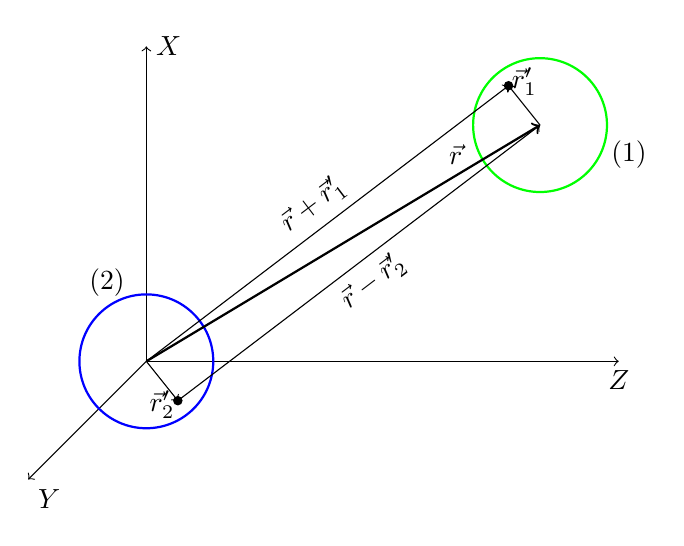
\begin{tikzpicture}
    \draw [->] (0, 0) -- (6, 0) node [anchor = north] {$Z$};
    \draw [->] (0, 0) -- (0, 4) node [anchor = west] {$X$};
    \draw [->] (0, 0) -- (-1.5, -1.5) node [anchor = north west] {$Y$};
    \draw [thick, blue] (0, 0) circle(0.85cm);
    \draw [thick, green] (5, 3) circle (0.85cm);
    \filldraw [black] (0.4, -0.5) circle (1.5pt);
    \filldraw [black] (4.6, 3.5) circle (1.5pt);
    \draw [->, thick] (0,0) -- (5, 3);
    \node [] at (3.93, 2.62) {$\vec{r}$};
    \draw [->] (0,0) -- (4.6, 3.5) node [midway, above, sloped] {$\vec{r} + \vec{r}_1'$};
    \draw [->] (0.4, -0.5) -- (5, 3) node [midway, below, sloped] {$\vec{r} - \vec{r}_2'$};
    \draw [->] (5,3) -- (4.6, 3.5) node [midway, above] {$\vec{r}_1'$};
    \draw [->] (0,0) -- (0.4, -0.5) node [midway, below,] {$\vec{r}_2'$};
    \node [] at (-0.5, 1) {(2)};
    \node [] at (6.13, 2.62) {(1)};
\end{tikzpicture}
            \caption{Взаимодействие двух систем}
        }
    \end{figure}

    Рассмотрим две системы зарядов на большом удалении друг от друга: $r \gg l_1, \: l_2$, где $r_{1,2}' \sim l_{1,2}$ --- характерные размеры систем.
    Найдём мультипольное разложение энергии взаимодействия:
    \begin{gather*}
        U_{12} = \int\rho(\vec{r} + \vec{r'})\phee{\vec{r} + \vec{r'}}d^2\vec{r'} \approx
        \int\rho(\vec{r} + \vec{r'}) \cdot \braces{\phee(\vec{r}) + \dotp{r}{\nabla} \phee(\vec{r}) + \frac{x_{\alpha}'x_{\beta}'}{2} \mixd{\phee}{x_{\alpha}}{x_{\beta}}} d^3\vec{r'}.
    \end{gather*}
    Вместо $\frac{x_{\alpha}'x_{\beta}'}{2}$ можно подставить $\frac 16 \brackets{3x_{\alpha}'x_{\beta}' - \delta_{\alpha\beta}(r')^2}$, потому что
    \[
        \delta_{\alpha\beta}\mixd{\phee}{x_{\alpha}}{x_{\beta}} = \mixd{\phee}{x_{\alpha}}{x_{\alpha}} = \Delta\phee.
    \]
    Вообще говоря, $\Delta\phee = 4\pi\rho$. Но у нас $U_{12} = \int\rho_1\phee_2 d\vol = \int\rho_2\phee_1 d\vol$ --- речь идёт о потенциале системы (1) в области системы (2) (или наоборот),
    а плотность зарядов системы (1) в области системы (2) равна нулю. Значит,
    \begin{gather*}
        \frac 16 \brackets{3x_{\alpha}'x_{\beta}' - \delta_{\alpha\beta}(r')^2} \mixd{\phee}{x_{\alpha}}{x_{\beta}} = \\
        = \frac{x_{\alpha}'x_{\beta}'}{2} \mixd{\phee}{x_{\alpha}}{x_{\beta}} - \frac 16 (r')^2 \Delta\phee = \frac{x_{\alpha}'x_{\beta}'}{2} \mixd{\phee}{x_{\alpha}}{x_{\beta}}.
    \end{gather*}
    С учётом подстановки проинтегрируем последнее слагаемое в разложении:
    \begin{gather*}
        \int \rho(\vec{r} + \vec{r'}) \frac{x_{\alpha}'x_{\beta}'}{2} \mixd{\phee}{x_{\alpha}}{x_{\beta}} d^3\vec{r'} = \\
        = \frac 16\int \rho(\vec{r} + \vec{r'}) \brackets{3x_{\alpha}'x_{\beta}' - \delta_{\alpha\beta}(r')^2} d^3\vec{r'} \mixd{\phee}{x_{\alpha}}{x_{\beta}} = \\
        = \frac 16 D_{\alpha\beta} \mixd{\phee}{x_{\alpha}}{x_{\beta}}.
    \end{gather*}
    Интегрируя остальные слагаемые, получаем окончательный ответ:
    \[
        U_{12} \approx e\phee(\vec{r}) - \brackets{\vec{d}\cdot\vec{E}(\vec{r})} + \frac 16 D_{\alpha\beta} \mixd{\phee}{x_{\alpha}}{x_{\beta}}.
    \]

    \begin{example} Энергия диполь-дипольного взаимодействия 
        (т. е. двух электронейтральных систем с ненулевым дипольным моментом). В энергии уднржим дипольное слагаемое,
        пренебрегая (если оно есть) квадрупольным:
        \[
            U_{12} = - \brackets{\vec{d}_1 \cdot \vec{E}_2};
        \]
        Поле диполя:
        \[
            \vec{E}_2 = \frac{-\vec{d}_2 + 3\dotp{d_2}{n}\vec{n}}{r^3},
        \]
        Откуда
        \[
            U_{12} = \frac{\dotp{d_1}{d_2} - 3\dotp{d_1}{n}\dotp{d_2}{n}}{r^3}.
        \]
        Градиент потенциальной энергии, как известно, есть сила взаимодействия:
        \[
            \vec{F} = -\nabla U = \nabla\dotp{d}{E} = \dotp{d}{\nabla}\vec{E}.
        \]
    \end{example}

\subsection{Уравнения магнитостатики}
    Вот они, слева направо:
    \[
        \rot\vec{H} = \frac{4\pi}{c}\vec{j}; \:\:\: \Div\vec{H} = 0.
    \]
    Так как магнитное поле создатся движущимися зарядами и действует также исключительно на движущиеся заряды, вообще говоря,
    под величинами $\vec{H}$ и $\vec{j}$ следует понимать их усреднённые по времени значения $\overline{\vec{H}}$ и $\overline{\vec{j}}$.
    Под магнитостатикой понимают отсутствие зависимости от времени в среднем, в этом случае $\Div\medv{j} = 0$, $\medv{H} = \rot\medv{A}$.
    
    В начале главы в условиях кулоновской калибровки мы получили уравнение Пуассона для магнитного поля (\ref{mag_Poisson}):
    \[
        \Delta\medv{A} = -\frac{4\pi}{c}\medv{j}.
    \]
    Решение этого уравнения полностью аналогично электростатическому:
    \[
        \medv{A}(\vec{r}) = \frac{1}{c}\int \frac{\medv{j}(\vec{r'})d\vol'}{\abs{\vec{r} - \vec{r'}}} = 
        \frac 1c \int G(\vec{r} - \vec{r'})\medv{j}(\vec{r'})v\vol'.
    \]
    где $G(\vec{r} - \vec{r'})$ --- \textit{функция Грина} уравнения Пуассона, в электростатическом имеющая смысл отклика на малый точечный заряд.
    Этот отклик суммируется по всему пространству с взвешиванием значением плотности заряда в каждой точке пространства.
    Функция Грина должна подчиняться уравнению
    $\Delta G(\vec{r} - \vec{r'}) = -4\pi\delta(\vec{r} - \vec{r'})$.
    Проверим, что выполняется условие $\Div\medv{A} = 0$:
    \begin{gather*}
        \Div\medv{A}(\vec{r}) = \frac 1c \int \brackets{\medv{j}(\vec{r'}) \cdot \vec{\nabla}_{\vec{r'}}}\frac{1}{\abs{\vec{r} - \vec{r'}}}d\vol' = \\ =
        -\frac 1c \int \Div_{\vec{r'}}\brackets{\frac{\medv{j}(\vec{r'})}{\abs{\vec{r} - \vec{r'}}}}d\vol' + 
        \frac 1c \int\frac{\Div_{\vec{r'}}\medv{j}(\vec{r'})}{\abs{\vec{r} - \vec{r'}}}d\vol'.
    \end{gather*}
    Второй член равен нулю в силу равенства $\Div\medv{j} = 0$, первый сводится к интегралу по поверхности в силу теоремы Гаусса-Остроградского
    и также равен нулю.

    Зная решение для векторного потенциала, можно найти магнитное поле и получить закон Био-Савара-Лапласа:
    \begin{gather*}
        \medv{H} = \rot\medv{A} = \frac 1c \int \sqbrk{\nabla\frac{1}{\abs{\vec{r} - \vec{r'}}} \times \medv{j}(\vec{r'})}d\vol' = \\ =
        \frac 1c \int \frac{\sqbrk{\medv{j}(\vec{r'}) \times \brackets{\vec{r} - \vec{r'}}}}{\abs{\vec{r} - \vec{r'}}^3}d\vol'
    \end{gather*}

    Рассмотрим поле на больших расстояниях от системы. Воспользуемся формулой
    \begin{gather*}
        \vec{A} = \frac 1c \int \frac{\vec{j}(\vec{r'})d\vol'}{\abs{\vec{r} - \vec{r'}}} = 
        \frac 1c \int \frac{\sum_ae_a\vec{v}_a\delta(\vec{r} - \vec{r}_a)}{\abs{\vec{r} - \vec{r'}}}d\vol' = \\ =
        \frac 1c \sum_a \frac{e_a\vec{v}_a}{\abs{\vec{r} - \vec{r'}}}.
    \end{gather*}
    Разложим знаменатель до второго порядка:
    \[
        \frac{1}{\abs{\vec{r} - \vec{r'}}} = \frac{1}{\sqrt{r^2 -2\dotp{r}{r_a} + r_a^2}} \approx \frac 1r \brackets{1 + \frac{\dotp{r}{r_a}}{r^2}}.
    \]
    Тогда, усредняя по времени:
    \begin{gather*}
        \medv{A}(\vec{r}) = \frac{1}{cr}\sum_a\overline{e_a\vec{v}_a + \frac{e_a\vec{v}_a \dotp{r}{r_a}}{r^2}}.
    \end{gather*}
    Так как система ограничена, то ограниченной является каждая из функций $\vec{r}_a(t)$. А так как усреднённая производная от 
    ограниченной функции есть ноль, то $e_a\vec{v_a} = \frac{d}{dt}\brackets{e_a\vec{r_a}} = 0$:
    \[
        \medv{A} = \frac{1}{cr^3}\sum_a\overline{e_a\vec{v}_a\dotp{r}{r_a}}.
    \]
    Используем соотношение
    \[
        \frac 12 \frac{d}{dt}\braces{\vec{r}_a \dotp{r}{r_a}} = \frac 12 \vec{v}_a \dotp{r}{r_a} + \frac 12 \vec{r}_a\dotp{r}{v_a},
    \]
    чтобы преобразовать выражение под знаком суммы:
    \[
        \medv{A} = \frac{1}{cr^3}\sum_a\overline{e_a\braces{\frac 12 \frac{d}{dt} 
        \brackets{\vec{r_a}\dotp{r}{r_a}} + \frac 12 \brackets{\vec{v_a}\dotp{r}{r_a}} - \vec{r_a}\dotp{v_a}{r_a}}}.
    \]
    Первое слагаемое в формуле равно нулю по той же причине. Сворачивая остальные по формуле двойного векторного произведения:
    \[
        \medv{A} = \frac{1}{2cr^3}\sum_a\overline{e_a\sqbrk{\vecp{r_a}{v_a} \times \vec{r}}}.
    \]
    По определению, $\frac{1}{2c} \overline{\sum_ae_a \vecp{r_a}{v_a}} = \vec{m}$ --- магнитный момент системы.
    Окончательно, поле на большом расстоянии от системы стационарно движущихся зарядов равно
    \[
        \boxed{\medv{A}(\vec{r}) = \frac{\vecp{m}{r}}{r^3}}
    \]
    Приведём также формулу поля такого магнитного диполя:
    \begin{gather*}
        \medv{H}(\vec{r}) = \rot\medv{A} = \rot\frac{\vecp{m}{r}}{r^3} = \frac{\rot\vecp{m}{r}}{r^3} + 
        \sqbrk{\nabla\frac{1}{r^3} \times \vecp{m}{r}} = \\ =
        \frac{2\vec{m}}{r^3} - \frac{3\sqbrk{\vec{r} \times \vecp{m}{r}}}{r^5} = \frac{3\dotp{m}{n}\vec{n} - \vec{m}}{r^3}.
    \end{gather*}